\documentclass[twoside]{book}

% Packages required by doxygen
\usepackage{fixltx2e}
\usepackage{calc}
\usepackage{doxygen}
\usepackage[export]{adjustbox} % also loads graphicx
\usepackage{graphicx}
\usepackage[utf8]{inputenc}
\usepackage{makeidx}
\usepackage{multicol}
\usepackage{multirow}
\PassOptionsToPackage{warn}{textcomp}
\usepackage{textcomp}
\usepackage[nointegrals]{wasysym}
\usepackage[table]{xcolor}

% Font selection
\usepackage[T1]{fontenc}
\usepackage[scaled=.90]{helvet}
\usepackage{courier}
\usepackage{amssymb}
\usepackage{sectsty}
\renewcommand{\familydefault}{\sfdefault}
\allsectionsfont{%
  \fontseries{bc}\selectfont%
  \color{darkgray}%
}
\renewcommand{\DoxyLabelFont}{%
  \fontseries{bc}\selectfont%
  \color{darkgray}%
}
\newcommand{\+}{\discretionary{\mbox{\scriptsize$\hookleftarrow$}}{}{}}

% Page & text layout
\usepackage{geometry}
\geometry{%
  a4paper,%
  top=2.5cm,%
  bottom=2.5cm,%
  left=2.5cm,%
  right=2.5cm%
}
\tolerance=750
\hfuzz=15pt
\hbadness=750
\setlength{\emergencystretch}{15pt}
\setlength{\parindent}{0cm}
\setlength{\parskip}{3ex plus 2ex minus 2ex}
\makeatletter
\renewcommand{\paragraph}{%
  \@startsection{paragraph}{4}{0ex}{-1.0ex}{1.0ex}{%
    \normalfont\normalsize\bfseries\SS@parafont%
  }%
}
\renewcommand{\subparagraph}{%
  \@startsection{subparagraph}{5}{0ex}{-1.0ex}{1.0ex}{%
    \normalfont\normalsize\bfseries\SS@subparafont%
  }%
}
\makeatother

% Headers & footers
\usepackage{fancyhdr}
\pagestyle{fancyplain}
\fancyhead[LE]{\fancyplain{}{\bfseries\thepage}}
\fancyhead[CE]{\fancyplain{}{}}
\fancyhead[RE]{\fancyplain{}{\bfseries\leftmark}}
\fancyhead[LO]{\fancyplain{}{\bfseries\rightmark}}
\fancyhead[CO]{\fancyplain{}{}}
\fancyhead[RO]{\fancyplain{}{\bfseries\thepage}}
\fancyfoot[LE]{\fancyplain{}{}}
\fancyfoot[CE]{\fancyplain{}{}}
\fancyfoot[RE]{\fancyplain{}{\bfseries\scriptsize Generated by Doxygen }}
\fancyfoot[LO]{\fancyplain{}{\bfseries\scriptsize Generated by Doxygen }}
\fancyfoot[CO]{\fancyplain{}{}}
\fancyfoot[RO]{\fancyplain{}{}}
\renewcommand{\footrulewidth}{0.4pt}
\renewcommand{\chaptermark}[1]{%
  \markboth{#1}{}%
}
\renewcommand{\sectionmark}[1]{%
  \markright{\thesection\ #1}%
}

% Indices & bibliography
\usepackage{natbib}
\usepackage[titles]{tocloft}
\setcounter{tocdepth}{3}
\setcounter{secnumdepth}{5}
\makeindex

% Hyperlinks (required, but should be loaded last)
\usepackage{ifpdf}
\ifpdf
  \usepackage[pdftex,pagebackref=true]{hyperref}
\else
  \usepackage[ps2pdf,pagebackref=true]{hyperref}
\fi
\hypersetup{%
  colorlinks=true,%
  linkcolor=blue,%
  citecolor=blue,%
  unicode%
}

% Custom commands
\newcommand{\clearemptydoublepage}{%
  \newpage{\pagestyle{empty}\cleardoublepage}%
}

\usepackage{caption}
\captionsetup{labelsep=space,justification=centering,font={bf},singlelinecheck=off,skip=4pt,position=top}

%===== C O N T E N T S =====

\begin{document}

% Titlepage & ToC
\hypersetup{pageanchor=false,
             bookmarksnumbered=true,
             pdfencoding=unicode
            }
\pagenumbering{alph}
\begin{titlepage}
\vspace*{7cm}
\begin{center}%
{\Large Human Detector and Tracker }\\
\vspace*{1cm}
{\large Generated by Doxygen 1.8.13}\\
\end{center}
\end{titlepage}
\clearemptydoublepage
\pagenumbering{roman}
\tableofcontents
\clearemptydoublepage
\pagenumbering{arabic}
\hypersetup{pageanchor=true}

%--- Begin generated contents ---
\chapter{Class Index}
\section{Class List}
Here are the classes, structs, unions and interfaces with brief descriptions\+:\begin{DoxyCompactList}
\item\contentsline{section}{\hyperlink{classHumanDetector}{Human\+Detector} \\*\hyperlink{classHumanDetector}{Human\+Detector} Class A class for human detection and drawing bounding boxes }{\pageref{classHumanDetector}}{}
\item\contentsline{section}{\hyperlink{classRobot}{Robot} \\*\hyperlink{classRobot}{Robot} class }{\pageref{classRobot}}{}
\end{DoxyCompactList}

\chapter{File Index}
\section{File List}
Here is a list of all documented files with brief descriptions\+:\begin{DoxyCompactList}
\item\contentsline{section}{include/\hyperlink{HumanDetector_8h}{Human\+Detector.\+h} }{\pageref{HumanDetector_8h}}{}
\item\contentsline{section}{include/\hyperlink{Robot_8h}{Robot.\+h} }{\pageref{Robot_8h}}{}
\item\contentsline{section}{src/\hyperlink{HumanDetector_8cpp}{Human\+Detector.\+cpp} }{\pageref{HumanDetector_8cpp}}{}
\item\contentsline{section}{src/\hyperlink{Robot_8cpp}{Robot.\+cpp} }{\pageref{Robot_8cpp}}{}
\end{DoxyCompactList}

\chapter{Class Documentation}
\hypertarget{classHumanDetector}{}\section{Human\+Detector Class Reference}
\label{classHumanDetector}\index{Human\+Detector@{Human\+Detector}}


\hyperlink{classHumanDetector}{Human\+Detector} Class A class for human detection and drawing bounding boxes.  




{\ttfamily \#include $<$Human\+Detector.\+h$>$}

\subsection*{Public Member Functions}
\begin{DoxyCompactItemize}
\item 
\hyperlink{classHumanDetector_a6a814e1705029576a7cb57a5727482e7}{Human\+Detector} (float conf\+\_\+th=0.\+6, float nms\+\_\+th=0.\+4)
\begin{DoxyCompactList}\small\item\em Construct a new Human Detector\+:\+: Human Detector object Set the thresholds for detection. \end{DoxyCompactList}\item 
void \hyperlink{classHumanDetector_aef7db39618f879d6e531e1f681553584}{set\+Confidence\+Threshold} (double conf\+\_\+th)
\begin{DoxyCompactList}\small\item\em Set confidence threshold for detection of humans. \end{DoxyCompactList}\item 
double \hyperlink{classHumanDetector_ae4d532d10e125e6f09f75896ddf37616}{get\+Confidence\+Threshold} ()
\begin{DoxyCompactList}\small\item\em Read the confidence threshold set in the A\+PI. \end{DoxyCompactList}\item 
void \hyperlink{classHumanDetector_a2120c8b55ea174c3742573ef9ed4549f}{set\+Nms\+Threshold} (double nms\+\_\+th)
\begin{DoxyCompactList}\small\item\em Set Non-\/maximum suppression threshold for detection of humans. \end{DoxyCompactList}\item 
double \hyperlink{classHumanDetector_a74f85f00e46601ceb2d6942e7ecf41eb}{get\+Nms\+Threshold} ()
\begin{DoxyCompactList}\small\item\em Read the Non-\/maximum suppression threshold set in the A\+PI. \end{DoxyCompactList}\item 
vector$<$ Mat $>$ \hyperlink{classHumanDetector_a54b25d621a57b068d4e069ce68ad944e}{detection} (Net \&net, Mat \&blob)
\begin{DoxyCompactList}\small\item\em detection \+: Runs the neural network to detect humans. \end{DoxyCompactList}\item 
vector$<$ Rect $>$ \hyperlink{classHumanDetector_a2246eb43446bfb27f8af71842b0e8215}{post\+Process} (Mat \&frame, const vector$<$ Mat $>$ \&outs)
\begin{DoxyCompactList}\small\item\em post\+Process \+: Performs confidence thresholding and non-\/max suppression. \end{DoxyCompactList}\item 
int \hyperlink{classHumanDetector_a798818fd11991551c1c6a68ae13f6321}{draw\+Bounding\+Boxes} (double confidence, int left, int top, int right, int bottom, Mat \&frame, int human\+\_\+number)
\begin{DoxyCompactList}\small\item\em draw\+Bounding\+Boxes \+: Draws bouding boxes around each human detected in frame. \end{DoxyCompactList}\item 
vector$<$ string $>$ \hyperlink{classHumanDetector_a0f42d17cfa9381ce20224fe3ffd25f28}{get\+Outputs\+Names} (const Net \&net)
\begin{DoxyCompactList}\small\item\em Get the Outputs Names object. \end{DoxyCompactList}\end{DoxyCompactItemize}


\subsection{Detailed Description}
\hyperlink{classHumanDetector}{Human\+Detector} Class A class for human detection and drawing bounding boxes. 

\subsection{Constructor \& Destructor Documentation}
\mbox{\Hypertarget{classHumanDetector_a6a814e1705029576a7cb57a5727482e7}\label{classHumanDetector_a6a814e1705029576a7cb57a5727482e7}} 
\index{Human\+Detector@{Human\+Detector}!Human\+Detector@{Human\+Detector}}
\index{Human\+Detector@{Human\+Detector}!Human\+Detector@{Human\+Detector}}
\subsubsection{\texorpdfstring{Human\+Detector()}{HumanDetector()}}
{\footnotesize\ttfamily Human\+Detector\+::\+Human\+Detector (\begin{DoxyParamCaption}\item[{float}]{conf\+\_\+th = {\ttfamily 0.6},  }\item[{float}]{nms\+\_\+th = {\ttfamily 0.4} }\end{DoxyParamCaption})\hspace{0.3cm}{\ttfamily [explicit]}}



Construct a new Human Detector\+:\+: Human Detector object Set the thresholds for detection. 


\begin{DoxyParams}{Parameters}
{\em conf\+\_\+th} & \+: Confidence threshold value \\
\hline
{\em nms\+\_\+th} & \+: N\+MS threshold value \\
\hline
\end{DoxyParams}


\subsection{Member Function Documentation}
\mbox{\Hypertarget{classHumanDetector_a54b25d621a57b068d4e069ce68ad944e}\label{classHumanDetector_a54b25d621a57b068d4e069ce68ad944e}} 
\index{Human\+Detector@{Human\+Detector}!detection@{detection}}
\index{detection@{detection}!Human\+Detector@{Human\+Detector}}
\subsubsection{\texorpdfstring{detection()}{detection()}}
{\footnotesize\ttfamily vector$<$ Mat $>$ Human\+Detector\+::detection (\begin{DoxyParamCaption}\item[{Net \&}]{net,  }\item[{Mat \&}]{blob }\end{DoxyParamCaption})}



detection \+: Runs the neural network to detect humans. 


\begin{DoxyParams}{Parameters}
{\em net} & \+: D\+NN network object \\
\hline
{\em blob} & \+: A 4D matrix \\
\hline
\end{DoxyParams}
\begin{DoxyReturn}{Returns}
vector$<$\+Mat$>$ A matrix with bounding boxes and scores 
\end{DoxyReturn}
\mbox{\Hypertarget{classHumanDetector_a798818fd11991551c1c6a68ae13f6321}\label{classHumanDetector_a798818fd11991551c1c6a68ae13f6321}} 
\index{Human\+Detector@{Human\+Detector}!draw\+Bounding\+Boxes@{draw\+Bounding\+Boxes}}
\index{draw\+Bounding\+Boxes@{draw\+Bounding\+Boxes}!Human\+Detector@{Human\+Detector}}
\subsubsection{\texorpdfstring{draw\+Bounding\+Boxes()}{drawBoundingBoxes()}}
{\footnotesize\ttfamily int Human\+Detector\+::draw\+Bounding\+Boxes (\begin{DoxyParamCaption}\item[{double}]{confidence,  }\item[{int}]{left,  }\item[{int}]{top,  }\item[{int}]{right,  }\item[{int}]{bottom,  }\item[{Mat \&}]{frame,  }\item[{int}]{human\+\_\+number }\end{DoxyParamCaption})}



draw\+Bounding\+Boxes \+: Draws bouding boxes around each human detected in frame. 


\begin{DoxyParams}{Parameters}
{\em confidence} & \+: Confidence for each detection \\
\hline
{\em left} & \+: bounding box dimension \\
\hline
{\em top} & \+: bounding box dimension \\
\hline
{\em right} & \+: bounding box dimension \\
\hline
{\em bottom} & \+: bounding box dimension \\
\hline
{\em frame} & \+: Current camera frame \\
\hline
{\em human\+\_\+number} & \+: Number of humans detected \\
\hline
\end{DoxyParams}
\begin{DoxyReturn}{Returns}
int \+: flag for indication 
\end{DoxyReturn}
\mbox{\Hypertarget{classHumanDetector_ae4d532d10e125e6f09f75896ddf37616}\label{classHumanDetector_ae4d532d10e125e6f09f75896ddf37616}} 
\index{Human\+Detector@{Human\+Detector}!get\+Confidence\+Threshold@{get\+Confidence\+Threshold}}
\index{get\+Confidence\+Threshold@{get\+Confidence\+Threshold}!Human\+Detector@{Human\+Detector}}
\subsubsection{\texorpdfstring{get\+Confidence\+Threshold()}{getConfidenceThreshold()}}
{\footnotesize\ttfamily double Human\+Detector\+::get\+Confidence\+Threshold (\begin{DoxyParamCaption}{ }\end{DoxyParamCaption})}



Read the confidence threshold set in the A\+PI. 

\begin{DoxyReturn}{Returns}
double \+: Confidence threshold 
\end{DoxyReturn}
\mbox{\Hypertarget{classHumanDetector_a74f85f00e46601ceb2d6942e7ecf41eb}\label{classHumanDetector_a74f85f00e46601ceb2d6942e7ecf41eb}} 
\index{Human\+Detector@{Human\+Detector}!get\+Nms\+Threshold@{get\+Nms\+Threshold}}
\index{get\+Nms\+Threshold@{get\+Nms\+Threshold}!Human\+Detector@{Human\+Detector}}
\subsubsection{\texorpdfstring{get\+Nms\+Threshold()}{getNmsThreshold()}}
{\footnotesize\ttfamily double Human\+Detector\+::get\+Nms\+Threshold (\begin{DoxyParamCaption}{ }\end{DoxyParamCaption})}



Read the Non-\/maximum suppression threshold set in the A\+PI. 

\begin{DoxyReturn}{Returns}
double \+: Non-\/maximum suppression threshold 
\end{DoxyReturn}
\mbox{\Hypertarget{classHumanDetector_a0f42d17cfa9381ce20224fe3ffd25f28}\label{classHumanDetector_a0f42d17cfa9381ce20224fe3ffd25f28}} 
\index{Human\+Detector@{Human\+Detector}!get\+Outputs\+Names@{get\+Outputs\+Names}}
\index{get\+Outputs\+Names@{get\+Outputs\+Names}!Human\+Detector@{Human\+Detector}}
\subsubsection{\texorpdfstring{get\+Outputs\+Names()}{getOutputsNames()}}
{\footnotesize\ttfamily vector$<$ string $>$ Human\+Detector\+::get\+Outputs\+Names (\begin{DoxyParamCaption}\item[{const Net \&}]{net }\end{DoxyParamCaption})}



Get the Outputs Names object. 


\begin{DoxyParams}{Parameters}
{\em net} & \+: Network to be used for detection \\
\hline
\end{DoxyParams}
\begin{DoxyReturn}{Returns}
vector$<$string$>$ \+: The names of output names 
\end{DoxyReturn}
\mbox{\Hypertarget{classHumanDetector_a2246eb43446bfb27f8af71842b0e8215}\label{classHumanDetector_a2246eb43446bfb27f8af71842b0e8215}} 
\index{Human\+Detector@{Human\+Detector}!post\+Process@{post\+Process}}
\index{post\+Process@{post\+Process}!Human\+Detector@{Human\+Detector}}
\subsubsection{\texorpdfstring{post\+Process()}{postProcess()}}
{\footnotesize\ttfamily vector$<$ Rect $>$ Human\+Detector\+::post\+Process (\begin{DoxyParamCaption}\item[{Mat \&}]{frame,  }\item[{const vector$<$ Mat $>$ \&}]{outs }\end{DoxyParamCaption})}



post\+Process \+: Performs confidence thresholding and non-\/max suppression. 


\begin{DoxyParams}{Parameters}
{\em frame} & \+: Current camera frame \\
\hline
{\em outs} & \+: A matrix with bounding boxes and scores \\
\hline
\end{DoxyParams}
\begin{DoxyReturn}{Returns}
vector$<$\+Rect$>$ \+: Dimensions of the bounding boxes for each human detected in frame. 
\end{DoxyReturn}
Later, it should return the x-\/axis of the bounding boxes for depth for transformation\mbox{\Hypertarget{classHumanDetector_aef7db39618f879d6e531e1f681553584}\label{classHumanDetector_aef7db39618f879d6e531e1f681553584}} 
\index{Human\+Detector@{Human\+Detector}!set\+Confidence\+Threshold@{set\+Confidence\+Threshold}}
\index{set\+Confidence\+Threshold@{set\+Confidence\+Threshold}!Human\+Detector@{Human\+Detector}}
\subsubsection{\texorpdfstring{set\+Confidence\+Threshold()}{setConfidenceThreshold()}}
{\footnotesize\ttfamily void Human\+Detector\+::set\+Confidence\+Threshold (\begin{DoxyParamCaption}\item[{double}]{conf\+\_\+th }\end{DoxyParamCaption})}



Set confidence threshold for detection of humans. 


\begin{DoxyParams}{Parameters}
{\em conf\+\_\+th} & \+: The value of confidence threshold \\
\hline
\end{DoxyParams}
\mbox{\Hypertarget{classHumanDetector_a2120c8b55ea174c3742573ef9ed4549f}\label{classHumanDetector_a2120c8b55ea174c3742573ef9ed4549f}} 
\index{Human\+Detector@{Human\+Detector}!set\+Nms\+Threshold@{set\+Nms\+Threshold}}
\index{set\+Nms\+Threshold@{set\+Nms\+Threshold}!Human\+Detector@{Human\+Detector}}
\subsubsection{\texorpdfstring{set\+Nms\+Threshold()}{setNmsThreshold()}}
{\footnotesize\ttfamily void Human\+Detector\+::set\+Nms\+Threshold (\begin{DoxyParamCaption}\item[{double}]{nms\+\_\+th }\end{DoxyParamCaption})}



Set Non-\/maximum suppression threshold for detection of humans. 


\begin{DoxyParams}{Parameters}
{\em nms\+\_\+th} & \+: The value of Non-\/maximum suppression threshold \\
\hline
\end{DoxyParams}


The documentation for this class was generated from the following files\+:\begin{DoxyCompactItemize}
\item 
include/\hyperlink{HumanDetector_8h}{Human\+Detector.\+h}\item 
src/\hyperlink{HumanDetector_8cpp}{Human\+Detector.\+cpp}\end{DoxyCompactItemize}

\hypertarget{classRobot}{}\section{Robot Class Reference}
\label{classRobot}\index{Robot@{Robot}}


\hyperlink{classRobot}{Robot} class.  




{\ttfamily \#include $<$Robot.\+h$>$}

\subsection*{Public Member Functions}
\begin{DoxyCompactItemize}
\item 
\hyperlink{classRobot_ad99a1ce9846d6334c2d9e9f52bbadce2}{Robot} (Matrix4d transformation\+\_\+matrix, double f\+\_\+length=984.\+251, double p\+\_\+height\+\_\+of\+\_\+human=672)
\begin{DoxyCompactList}\small\item\em Construct a new \hyperlink{classRobot}{Robot}\+:\+: \hyperlink{classRobot}{Robot} object. \end{DoxyCompactList}\item 
Net \hyperlink{classRobot_a082dee8da5e4847ded0a6a1373172073}{load\+Network} (string model\+\_\+config, string model\+\_\+weights)
\begin{DoxyCompactList}\small\item\em Load the pre trained network using weights and configurations. \end{DoxyCompactList}\item 
double \hyperlink{classRobot_ad5b286958dbf40329f8cebdb9c9c4987}{get\+Focal\+Length} ()
\begin{DoxyCompactList}\small\item\em Read the focal length defined in the A\+PI. \end{DoxyCompactList}\item 
void \hyperlink{classRobot_aad2cd63f57d4feaaa7ec92f49ba72d5e}{set\+Focal\+Length} (double focal\+\_\+length)
\begin{DoxyCompactList}\small\item\em Set focal length of the camera being used. \end{DoxyCompactList}\item 
vector$<$ int $>$ \hyperlink{classRobot_a3a1999a77bc11f070daaa0655ddff66b}{get\+Shape} ()
\begin{DoxyCompactList}\small\item\em Read the size of the input used for the network. \end{DoxyCompactList}\item 
void \hyperlink{classRobot_a2362bcfbd845f451a278b3d6af907f1f}{set\+Transformation\+Matrix} (Eigen\+::\+Matrix4d matrix)
\begin{DoxyCompactList}\small\item\em Set the transformation matrix for getting the location of human detected from camera\textquotesingle{}s reference frame to robot\textquotesingle{}s reference frame. \end{DoxyCompactList}\item 
Eigen\+::\+Matrix4d \hyperlink{classRobot_a0034f52a4daac582470860655f38f734}{get\+Transformation\+Matrix} ()
\begin{DoxyCompactList}\small\item\em Read the transformation matrix for getting the location of human detected from camera\textquotesingle{}s reference frame to robot\textquotesingle{}s reference frame. \end{DoxyCompactList}\item 
Mat \hyperlink{classRobot_a16845345490d84f599e5b469eca208dd}{prep\+Frame} (Mat frame)
\begin{DoxyCompactList}\small\item\em prep\+Frame \+: Pre processing of the camera frame \end{DoxyCompactList}\item 
double \hyperlink{classRobot_a7d7c5ba1d9b83dcb6bc6413d7b89c6ff}{calculate\+Depth} (Rect bbox\+\_\+coords)
\begin{DoxyCompactList}\small\item\em Calculate the depth of the person being detected in frame. \end{DoxyCompactList}\item 
vector$<$ Rect $>$ \hyperlink{classRobot_a090b8f765b5d83a322576fb9d48bb14e}{transform\+To\+Robot\+Frame} (vector$<$ Rect $>$ bbox\+\_\+coords)
\begin{DoxyCompactList}\small\item\em Convert the location of human detected from camera\textquotesingle{}s reference frame to robot\textquotesingle{}s reference frame. \end{DoxyCompactList}\item 
vector$<$ Rect $>$ \hyperlink{classRobot_ab98ffeccb3b37392f4336e3a6dd14913}{detect\+Humans} (Mat frame, Net net)
\begin{DoxyCompactList}\small\item\em Detect humans in given frame and get the location of each human in robot\textquotesingle{}s reference frame. \end{DoxyCompactList}\end{DoxyCompactItemize}


\subsection{Detailed Description}
\hyperlink{classRobot}{Robot} class. 

\subsection{Constructor \& Destructor Documentation}
\mbox{\Hypertarget{classRobot_ad99a1ce9846d6334c2d9e9f52bbadce2}\label{classRobot_ad99a1ce9846d6334c2d9e9f52bbadce2}} 
\index{Robot@{Robot}!Robot@{Robot}}
\index{Robot@{Robot}!Robot@{Robot}}
\subsubsection{\texorpdfstring{Robot()}{Robot()}}
{\footnotesize\ttfamily Robot\+::\+Robot (\begin{DoxyParamCaption}\item[{Matrix4d}]{transformation\+\_\+matrix,  }\item[{double}]{f\+\_\+length = {\ttfamily 984.251},  }\item[{double}]{p\+\_\+height\+\_\+of\+\_\+human = {\ttfamily 672} }\end{DoxyParamCaption})\hspace{0.3cm}{\ttfamily [explicit]}}



Construct a new \hyperlink{classRobot}{Robot}\+:\+: \hyperlink{classRobot}{Robot} object. 


\begin{DoxyParams}{Parameters}
{\em transformation\+\_\+matrix} & \+: The transformation matrix for getting the location of human detected from camera\textquotesingle{}s reference frame to robot\textquotesingle{}s reference frame. \\
\hline
{\em f\+\_\+length} & \+: Focal length of the camera being using. \\
\hline
{\em p\+\_\+height\+\_\+of\+\_\+human} & \+: Height of the human in pixel. \\
\hline
\end{DoxyParams}


\subsection{Member Function Documentation}
\mbox{\Hypertarget{classRobot_a7d7c5ba1d9b83dcb6bc6413d7b89c6ff}\label{classRobot_a7d7c5ba1d9b83dcb6bc6413d7b89c6ff}} 
\index{Robot@{Robot}!calculate\+Depth@{calculate\+Depth}}
\index{calculate\+Depth@{calculate\+Depth}!Robot@{Robot}}
\subsubsection{\texorpdfstring{calculate\+Depth()}{calculateDepth()}}
{\footnotesize\ttfamily double Robot\+::calculate\+Depth (\begin{DoxyParamCaption}\item[{Rect}]{bbox\+\_\+coords }\end{DoxyParamCaption})}



Calculate the depth of the person being detected in frame. 


\begin{DoxyParams}{Parameters}
{\em bbox\+\_\+coords} & \+: The 2D coordinates of the person being detected in frame \\
\hline
\end{DoxyParams}
\begin{DoxyReturn}{Returns}
double \+: the depth of the person being detected in frame 
\end{DoxyReturn}
\mbox{\Hypertarget{classRobot_ab98ffeccb3b37392f4336e3a6dd14913}\label{classRobot_ab98ffeccb3b37392f4336e3a6dd14913}} 
\index{Robot@{Robot}!detect\+Humans@{detect\+Humans}}
\index{detect\+Humans@{detect\+Humans}!Robot@{Robot}}
\subsubsection{\texorpdfstring{detect\+Humans()}{detectHumans()}}
{\footnotesize\ttfamily vector$<$ Rect $>$ Robot\+::detect\+Humans (\begin{DoxyParamCaption}\item[{Mat}]{frame,  }\item[{Net}]{net }\end{DoxyParamCaption})}



Detect humans in given frame and get the location of each human in robot\textquotesingle{}s reference frame. 


\begin{DoxyParams}{Parameters}
{\em frame} & \+: Current Camera frame \\
\hline
{\em net} & \+: Network for detection \\
\hline
\end{DoxyParams}
\begin{DoxyReturn}{Returns}
vector$<$\+Rect$>$ \+: Location of each human in robot\textquotesingle{}s reference frame 
\end{DoxyReturn}
\mbox{\Hypertarget{classRobot_ad5b286958dbf40329f8cebdb9c9c4987}\label{classRobot_ad5b286958dbf40329f8cebdb9c9c4987}} 
\index{Robot@{Robot}!get\+Focal\+Length@{get\+Focal\+Length}}
\index{get\+Focal\+Length@{get\+Focal\+Length}!Robot@{Robot}}
\subsubsection{\texorpdfstring{get\+Focal\+Length()}{getFocalLength()}}
{\footnotesize\ttfamily double Robot\+::get\+Focal\+Length (\begin{DoxyParamCaption}{ }\end{DoxyParamCaption})}



Read the focal length defined in the A\+PI. 

\begin{DoxyReturn}{Returns}
double The focal length set in the A\+PI. 
\end{DoxyReturn}
\mbox{\Hypertarget{classRobot_a3a1999a77bc11f070daaa0655ddff66b}\label{classRobot_a3a1999a77bc11f070daaa0655ddff66b}} 
\index{Robot@{Robot}!get\+Shape@{get\+Shape}}
\index{get\+Shape@{get\+Shape}!Robot@{Robot}}
\subsubsection{\texorpdfstring{get\+Shape()}{getShape()}}
{\footnotesize\ttfamily vector$<$ int $>$ Robot\+::get\+Shape (\begin{DoxyParamCaption}{ }\end{DoxyParamCaption})}



Read the size of the input used for the network. 

\begin{DoxyReturn}{Returns}
vector$<$int$>$ \+: Size of the input used for the network 
\end{DoxyReturn}
\mbox{\Hypertarget{classRobot_a0034f52a4daac582470860655f38f734}\label{classRobot_a0034f52a4daac582470860655f38f734}} 
\index{Robot@{Robot}!get\+Transformation\+Matrix@{get\+Transformation\+Matrix}}
\index{get\+Transformation\+Matrix@{get\+Transformation\+Matrix}!Robot@{Robot}}
\subsubsection{\texorpdfstring{get\+Transformation\+Matrix()}{getTransformationMatrix()}}
{\footnotesize\ttfamily Eigen\+::\+Matrix4d Robot\+::get\+Transformation\+Matrix (\begin{DoxyParamCaption}{ }\end{DoxyParamCaption})}



Read the transformation matrix for getting the location of human detected from camera\textquotesingle{}s reference frame to robot\textquotesingle{}s reference frame. 

\begin{DoxyReturn}{Returns}
Eigen\+::\+Matrix4d \+: Transformation matrix 
\end{DoxyReturn}
\mbox{\Hypertarget{classRobot_a082dee8da5e4847ded0a6a1373172073}\label{classRobot_a082dee8da5e4847ded0a6a1373172073}} 
\index{Robot@{Robot}!load\+Network@{load\+Network}}
\index{load\+Network@{load\+Network}!Robot@{Robot}}
\subsubsection{\texorpdfstring{load\+Network()}{loadNetwork()}}
{\footnotesize\ttfamily Net Robot\+::load\+Network (\begin{DoxyParamCaption}\item[{string}]{model\+\_\+config,  }\item[{string}]{model\+\_\+weights }\end{DoxyParamCaption})}



Load the pre trained network using weights and configurations. 


\begin{DoxyParams}{Parameters}
{\em model\+\_\+config} & \+: Configuration file of the model used. \\
\hline
{\em model\+\_\+weights} & \+: Pre trained weights of the model used. \\
\hline
\end{DoxyParams}
\begin{DoxyReturn}{Returns}
Net \+: Model being used. 
\end{DoxyReturn}
\mbox{\Hypertarget{classRobot_a16845345490d84f599e5b469eca208dd}\label{classRobot_a16845345490d84f599e5b469eca208dd}} 
\index{Robot@{Robot}!prep\+Frame@{prep\+Frame}}
\index{prep\+Frame@{prep\+Frame}!Robot@{Robot}}
\subsubsection{\texorpdfstring{prep\+Frame()}{prepFrame()}}
{\footnotesize\ttfamily Mat Robot\+::prep\+Frame (\begin{DoxyParamCaption}\item[{Mat}]{frame }\end{DoxyParamCaption})}



prep\+Frame \+: Pre processing of the camera frame 


\begin{DoxyParams}{Parameters}
{\em frame} & \+: Current Camera frame \\
\hline
\end{DoxyParams}
\begin{DoxyReturn}{Returns}
Mat \+: processed camera frame, ready for detection 
\end{DoxyReturn}
\mbox{\Hypertarget{classRobot_aad2cd63f57d4feaaa7ec92f49ba72d5e}\label{classRobot_aad2cd63f57d4feaaa7ec92f49ba72d5e}} 
\index{Robot@{Robot}!set\+Focal\+Length@{set\+Focal\+Length}}
\index{set\+Focal\+Length@{set\+Focal\+Length}!Robot@{Robot}}
\subsubsection{\texorpdfstring{set\+Focal\+Length()}{setFocalLength()}}
{\footnotesize\ttfamily void Robot\+::set\+Focal\+Length (\begin{DoxyParamCaption}\item[{double}]{f }\end{DoxyParamCaption})}



Set focal length of the camera being used. 


\begin{DoxyParams}{Parameters}
{\em f} & Focal length of the camera being used. \\
\hline
\end{DoxyParams}
\mbox{\Hypertarget{classRobot_a2362bcfbd845f451a278b3d6af907f1f}\label{classRobot_a2362bcfbd845f451a278b3d6af907f1f}} 
\index{Robot@{Robot}!set\+Transformation\+Matrix@{set\+Transformation\+Matrix}}
\index{set\+Transformation\+Matrix@{set\+Transformation\+Matrix}!Robot@{Robot}}
\subsubsection{\texorpdfstring{set\+Transformation\+Matrix()}{setTransformationMatrix()}}
{\footnotesize\ttfamily void Robot\+::set\+Transformation\+Matrix (\begin{DoxyParamCaption}\item[{Eigen\+::\+Matrix4d}]{matrix }\end{DoxyParamCaption})}



Set the transformation matrix for getting the location of human detected from camera\textquotesingle{}s reference frame to robot\textquotesingle{}s reference frame. 


\begin{DoxyParams}{Parameters}
{\em matrix} & \+: Transformation matrix \\
\hline
\end{DoxyParams}
\mbox{\Hypertarget{classRobot_a090b8f765b5d83a322576fb9d48bb14e}\label{classRobot_a090b8f765b5d83a322576fb9d48bb14e}} 
\index{Robot@{Robot}!transform\+To\+Robot\+Frame@{transform\+To\+Robot\+Frame}}
\index{transform\+To\+Robot\+Frame@{transform\+To\+Robot\+Frame}!Robot@{Robot}}
\subsubsection{\texorpdfstring{transform\+To\+Robot\+Frame()}{transformToRobotFrame()}}
{\footnotesize\ttfamily vector$<$ Rect $>$ Robot\+::transform\+To\+Robot\+Frame (\begin{DoxyParamCaption}\item[{vector$<$ Rect $>$}]{bbox\+\_\+coords }\end{DoxyParamCaption})}



Convert the location of human detected from camera\textquotesingle{}s reference frame to robot\textquotesingle{}s reference frame. 


\begin{DoxyParams}{Parameters}
{\em bbox\+\_\+coords} & \+: location of each human in camera reference frame \\
\hline
\end{DoxyParams}
\begin{DoxyReturn}{Returns}
vector$<$\+Rect$>$ \+: location of each human in robot reference frame 
\end{DoxyReturn}
Calculate location of point wrt robot frame using transformation matrix

The documentation for this class was generated from the following files\+:\begin{DoxyCompactItemize}
\item 
include/\hyperlink{Robot_8h}{Robot.\+h}\item 
src/\hyperlink{Robot_8cpp}{Robot.\+cpp}\end{DoxyCompactItemize}

\chapter{File Documentation}
\hypertarget{HumanDetector_8h}{}\section{include/\+Human\+Detector.h File Reference}
\label{HumanDetector_8h}\index{include/\+Human\+Detector.\+h@{include/\+Human\+Detector.\+h}}
{\ttfamily \#include $<$Eigen/\+Dense$>$}\newline
{\ttfamily \#include $<$iostream$>$}\newline
{\ttfamily \#include $<$vector$>$}\newline
{\ttfamily \#include $<$string$>$}\newline
{\ttfamily \#include $<$opencv2/dnn.\+hpp$>$}\newline
{\ttfamily \#include $<$opencv2/imgproc.\+hpp$>$}\newline
{\ttfamily \#include $<$opencv2/highgui.\+hpp$>$}\newline
Include dependency graph for Human\+Detector.\+h\+:\nopagebreak
\begin{figure}[H]
\begin{center}
\leavevmode
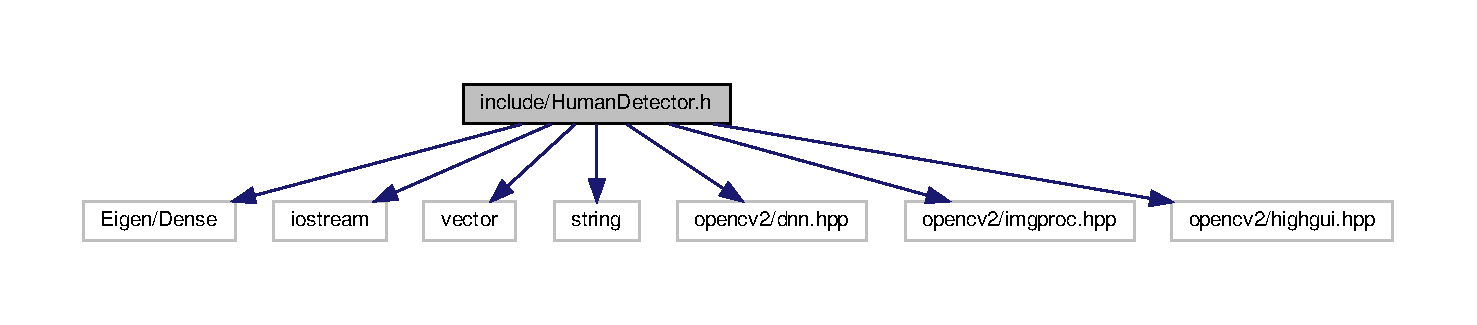
\includegraphics[width=350pt]{HumanDetector_8h__incl}
\end{center}
\end{figure}
This graph shows which files directly or indirectly include this file\+:\nopagebreak
\begin{figure}[H]
\begin{center}
\leavevmode
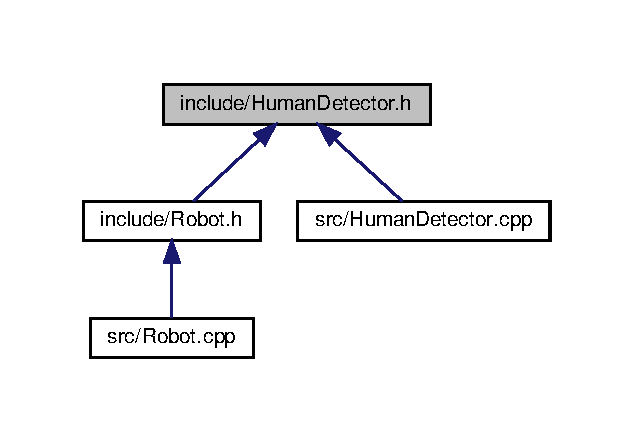
\includegraphics[width=304pt]{HumanDetector_8h__dep__incl}
\end{center}
\end{figure}
\subsection*{Classes}
\begin{DoxyCompactItemize}
\item 
class \hyperlink{classHumanDetector}{Human\+Detector}
\begin{DoxyCompactList}\small\item\em \hyperlink{classHumanDetector}{Human\+Detector} Class A class for human detection and drawing bounding boxes. \end{DoxyCompactList}\end{DoxyCompactItemize}


\subsection{Detailed Description}
Copyright (c) 2021 Aditi Ramadwar, Arunava Basu

Permission is hereby granted, free of charge, to any person obtaining a copy of this software and associated documentation files (the \char`\"{}\+Software\char`\"{}), to deal in the Software without restriction, including without limitation the rights to use, copy, modify, merge, publish, distribute, sublicense, and/or sell copies of the Software, and to permit persons to whom the Software is furnished to do so, subject to the following conditions\+:

The above copyright notice and this permission notice shall be included in all copies or substantial portions of the Software. T\+HE S\+O\+F\+T\+W\+A\+RE IS P\+R\+O\+V\+I\+D\+ED \char`\"{}\+A\+S I\+S\char`\"{}, W\+I\+T\+H\+O\+UT W\+A\+R\+R\+A\+N\+TY OF A\+NY K\+I\+ND, E\+X\+P\+R\+E\+SS OR I\+M\+P\+L\+I\+ED, I\+N\+C\+L\+U\+D\+I\+NG B\+UT N\+OT L\+I\+M\+I\+T\+ED TO T\+HE W\+A\+R\+R\+A\+N\+T\+I\+ES OF M\+E\+R\+C\+H\+A\+N\+T\+A\+B\+I\+L\+I\+TY, F\+I\+T\+N\+E\+SS F\+OR A P\+A\+R\+T\+I\+C\+U\+L\+AR P\+U\+R\+P\+O\+SE A\+ND N\+O\+N\+I\+N\+F\+R\+I\+N\+G\+E\+M\+E\+NT. IN NO E\+V\+E\+NT S\+H\+A\+LL T\+HE A\+U\+T\+H\+O\+RS OR C\+O\+P\+Y\+R\+I\+G\+HT H\+O\+L\+D\+E\+RS BE L\+I\+A\+B\+LE F\+OR A\+NY C\+L\+A\+IM, D\+A\+M\+A\+G\+ES OR O\+T\+H\+ER L\+I\+A\+B\+I\+L\+I\+TY, W\+H\+E\+T\+H\+ER IN AN A\+C\+T\+I\+ON OF C\+O\+N\+T\+R\+A\+CT, T\+O\+RT OR O\+T\+H\+E\+R\+W\+I\+SE, A\+R\+I\+S\+I\+NG F\+R\+OM, O\+UT OF OR IN C\+O\+N\+N\+E\+C\+T\+I\+ON W\+I\+TH T\+HE S\+O\+F\+T\+W\+A\+RE OR T\+HE U\+SE OR O\+T\+H\+ER D\+E\+A\+L\+I\+N\+GS IN T\+HE S\+O\+F\+T\+W\+A\+RE.

\begin{DoxyAuthor}{Author}
Iteration 1 \+: Aditi Ramadwar (Driver) , Arunava Basu (Navigator) Iteration 2 \+: Arunava Basu (Navigator) , Aditi Ramadwar (Driver) 
\end{DoxyAuthor}
\begin{DoxyVersion}{Version}
0.\+1 
\end{DoxyVersion}
\begin{DoxyDate}{Date}
2021-\/10-\/14
\end{DoxyDate}
\begin{DoxyCopyright}{Copyright}
Copyright (c) 2021 
\end{DoxyCopyright}

\hypertarget{Robot_8h}{}\section{include/\+Robot.h File Reference}
\label{Robot_8h}\index{include/\+Robot.\+h@{include/\+Robot.\+h}}
{\ttfamily \#include \char`\"{}Human\+Detector.\+h\char`\"{}}\newline
{\ttfamily \#include $<$vector$>$}\newline
{\ttfamily \#include $<$string$>$}\newline
Include dependency graph for Robot.\+h\+:\nopagebreak
\begin{figure}[H]
\begin{center}
\leavevmode
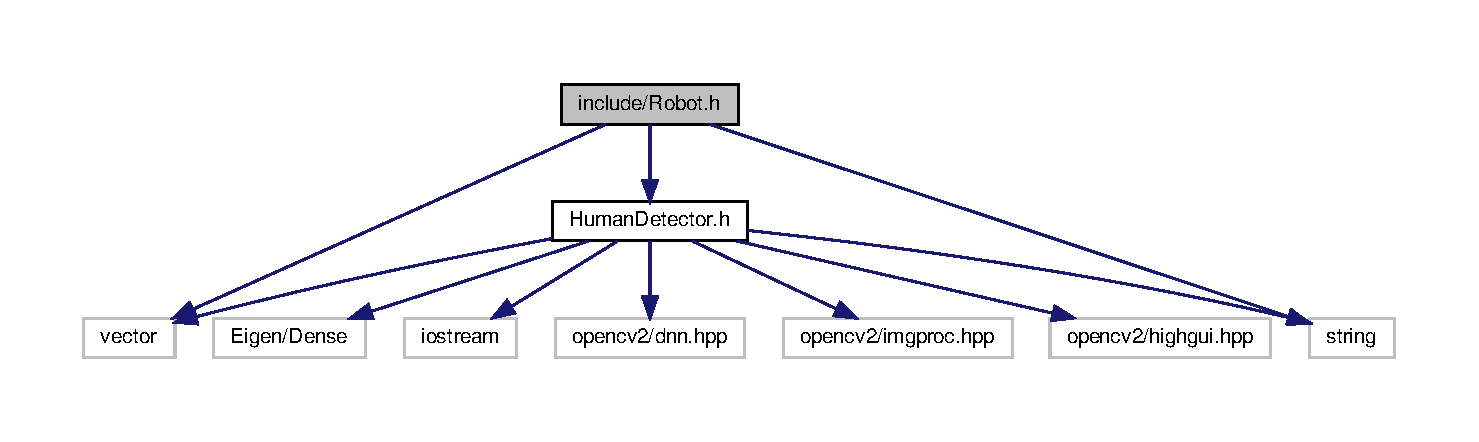
\includegraphics[width=350pt]{Robot_8h__incl}
\end{center}
\end{figure}
This graph shows which files directly or indirectly include this file\+:\nopagebreak
\begin{figure}[H]
\begin{center}
\leavevmode
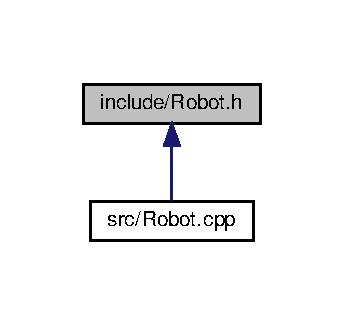
\includegraphics[width=165pt]{Robot_8h__dep__incl}
\end{center}
\end{figure}
\subsection*{Classes}
\begin{DoxyCompactItemize}
\item 
class \hyperlink{classRobot}{Robot}
\begin{DoxyCompactList}\small\item\em \hyperlink{classRobot}{Robot} class. \end{DoxyCompactList}\end{DoxyCompactItemize}


\subsection{Detailed Description}
Copyright (c) 2021 Aditi Ramadwar, Arunava Basu

Permission is hereby granted, free of charge, to any person obtaining a copy of this software and associated documentation files (the \char`\"{}\+Software\char`\"{}), to deal in the Software without restriction, including without limitation the rights to use, copy, modify, merge, publish, distribute, sublicense, and/or sell copies of the Software, and to permit persons to whom the Software is furnished to do so, subject to the following conditions\+:

The above copyright notice and this permission notice shall be included in all copies or substantial portions of the Software. T\+HE S\+O\+F\+T\+W\+A\+RE IS P\+R\+O\+V\+I\+D\+ED \char`\"{}\+A\+S I\+S\char`\"{}, W\+I\+T\+H\+O\+UT W\+A\+R\+R\+A\+N\+TY OF A\+NY K\+I\+ND, E\+X\+P\+R\+E\+SS OR I\+M\+P\+L\+I\+ED, I\+N\+C\+L\+U\+D\+I\+NG B\+UT N\+OT L\+I\+M\+I\+T\+ED TO T\+HE W\+A\+R\+R\+A\+N\+T\+I\+ES OF M\+E\+R\+C\+H\+A\+N\+T\+A\+B\+I\+L\+I\+TY, F\+I\+T\+N\+E\+SS F\+OR A P\+A\+R\+T\+I\+C\+U\+L\+AR P\+U\+R\+P\+O\+SE A\+ND N\+O\+N\+I\+N\+F\+R\+I\+N\+G\+E\+M\+E\+NT. IN NO E\+V\+E\+NT S\+H\+A\+LL T\+HE A\+U\+T\+H\+O\+RS OR C\+O\+P\+Y\+R\+I\+G\+HT H\+O\+L\+D\+E\+RS BE L\+I\+A\+B\+LE F\+OR A\+NY C\+L\+A\+IM, D\+A\+M\+A\+G\+ES OR O\+T\+H\+ER L\+I\+A\+B\+I\+L\+I\+TY, W\+H\+E\+T\+H\+ER IN AN A\+C\+T\+I\+ON OF C\+O\+N\+T\+R\+A\+CT, T\+O\+RT OR O\+T\+H\+E\+R\+W\+I\+SE, A\+R\+I\+S\+I\+NG F\+R\+OM, O\+UT OF OR IN C\+O\+N\+N\+E\+C\+T\+I\+ON W\+I\+TH T\+HE S\+O\+F\+T\+W\+A\+RE OR T\+HE U\+SE OR O\+T\+H\+ER D\+E\+A\+L\+I\+N\+GS IN T\+HE S\+O\+F\+T\+W\+A\+RE.

\begin{DoxyAuthor}{Author}
Iteration 1 \+: Aditi Ramadwar (Driver) , Arunava Basu (Navigator) Iteration 2 \+: Arunava Basu (Navigator) , Aditi Ramadwar (Driver) 
\end{DoxyAuthor}
\begin{DoxyVersion}{Version}
0.\+1 
\end{DoxyVersion}
\begin{DoxyDate}{Date}
2021-\/10-\/14
\end{DoxyDate}
\begin{DoxyCopyright}{Copyright}
Copyright (c) 2021 
\end{DoxyCopyright}

\hypertarget{HumanDetector_8cpp}{}\section{src/\+Human\+Detector.cpp File Reference}
\label{HumanDetector_8cpp}\index{src/\+Human\+Detector.\+cpp@{src/\+Human\+Detector.\+cpp}}
{\ttfamily \#include \char`\"{}Human\+Detector.\+h\char`\"{}}\newline
Include dependency graph for Human\+Detector.\+cpp\+:\nopagebreak
\begin{figure}[H]
\begin{center}
\leavevmode
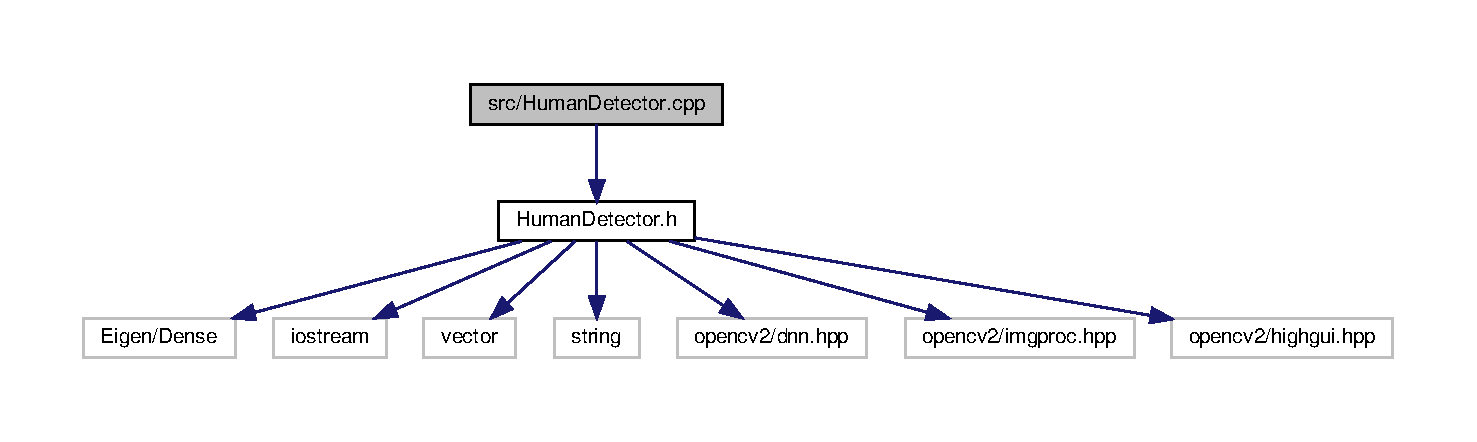
\includegraphics[width=350pt]{HumanDetector_8cpp__incl}
\end{center}
\end{figure}


\subsection{Detailed Description}
Copyright (c) 2021 Aditi Ramadwar, Arunava Basu

Permission is hereby granted, free of charge, to any person obtaining a copy of this software and associated documentation files (the \char`\"{}\+Software\char`\"{}), to deal in the Software without restriction, including without limitation the rights to use, copy, modify, merge, publish, distribute, sublicense, and/or sell copies of the Software, and to permit persons to whom the Software is furnished to do so, subject to the following conditions\+:

The above copyright notice and this permission notice shall be included in all copies or substantial portions of the Software. T\+HE S\+O\+F\+T\+W\+A\+RE IS P\+R\+O\+V\+I\+D\+ED \char`\"{}\+A\+S I\+S\char`\"{}, W\+I\+T\+H\+O\+UT W\+A\+R\+R\+A\+N\+TY OF A\+NY K\+I\+ND, E\+X\+P\+R\+E\+SS OR I\+M\+P\+L\+I\+ED, I\+N\+C\+L\+U\+D\+I\+NG B\+UT N\+OT L\+I\+M\+I\+T\+ED TO T\+HE W\+A\+R\+R\+A\+N\+T\+I\+ES OF M\+E\+R\+C\+H\+A\+N\+T\+A\+B\+I\+L\+I\+TY, F\+I\+T\+N\+E\+SS F\+OR A P\+A\+R\+T\+I\+C\+U\+L\+AR P\+U\+R\+P\+O\+SE A\+ND N\+O\+N\+I\+N\+F\+R\+I\+N\+G\+E\+M\+E\+NT. IN NO E\+V\+E\+NT S\+H\+A\+LL T\+HE A\+U\+T\+H\+O\+RS OR C\+O\+P\+Y\+R\+I\+G\+HT H\+O\+L\+D\+E\+RS BE L\+I\+A\+B\+LE F\+OR A\+NY C\+L\+A\+IM, D\+A\+M\+A\+G\+ES OR O\+T\+H\+ER L\+I\+A\+B\+I\+L\+I\+TY, W\+H\+E\+T\+H\+ER IN AN A\+C\+T\+I\+ON OF C\+O\+N\+T\+R\+A\+CT, T\+O\+RT OR O\+T\+H\+E\+R\+W\+I\+SE, A\+R\+I\+S\+I\+NG F\+R\+OM, O\+UT OF OR IN C\+O\+N\+N\+E\+C\+T\+I\+ON W\+I\+TH T\+HE S\+O\+F\+T\+W\+A\+RE OR T\+HE U\+SE OR O\+T\+H\+ER D\+E\+A\+L\+I\+N\+GS IN T\+HE S\+O\+F\+T\+W\+A\+RE.

\begin{DoxyAuthor}{Author}
Iteration 1 \+: Aditi Ramadwar (Driver) , Arunava Basu (Navigator) Iteration 2 \+: Arunava Basu (Navigator) , Aditi Ramadwar (Driver) 
\end{DoxyAuthor}
\begin{DoxyVersion}{Version}
0.\+1 
\end{DoxyVersion}
\begin{DoxyDate}{Date}
2021-\/10-\/14
\end{DoxyDate}
\begin{DoxyCopyright}{Copyright}
Copyright (c) 2021 
\end{DoxyCopyright}

\hypertarget{Robot_8cpp}{}\section{src/\+Robot.cpp File Reference}
\label{Robot_8cpp}\index{src/\+Robot.\+cpp@{src/\+Robot.\+cpp}}
{\ttfamily \#include \char`\"{}Robot.\+h\char`\"{}}\newline
Include dependency graph for Robot.\+cpp\+:\nopagebreak
\begin{figure}[H]
\begin{center}
\leavevmode
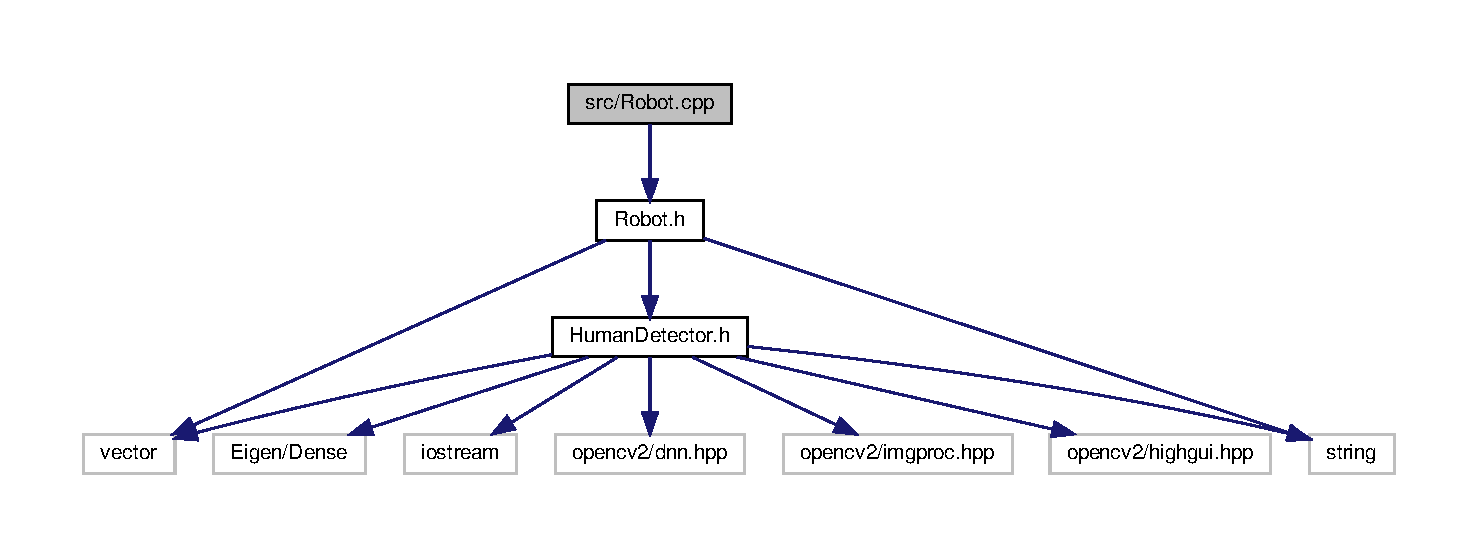
\includegraphics[width=350pt]{Robot_8cpp__incl}
\end{center}
\end{figure}


\subsection{Detailed Description}
Copyright (c) 2021 Aditi Ramadwar, Arunava Basu

Permission is hereby granted, free of charge, to any person obtaining a copy of this software and associated documentation files (the \char`\"{}\+Software\char`\"{}), to deal in the Software without restriction, including without limitation the rights to use, copy, modify, merge, publish, distribute, sublicense, and/or sell copies of the Software, and to permit persons to whom the Software is furnished to do so, subject to the following conditions\+:

The above copyright notice and this permission notice shall be included in all copies or substantial portions of the Software. T\+HE S\+O\+F\+T\+W\+A\+RE IS P\+R\+O\+V\+I\+D\+ED \char`\"{}\+A\+S I\+S\char`\"{}, W\+I\+T\+H\+O\+UT W\+A\+R\+R\+A\+N\+TY OF A\+NY K\+I\+ND, E\+X\+P\+R\+E\+SS OR I\+M\+P\+L\+I\+ED, I\+N\+C\+L\+U\+D\+I\+NG B\+UT N\+OT L\+I\+M\+I\+T\+ED TO T\+HE W\+A\+R\+R\+A\+N\+T\+I\+ES OF M\+E\+R\+C\+H\+A\+N\+T\+A\+B\+I\+L\+I\+TY, F\+I\+T\+N\+E\+SS F\+OR A P\+A\+R\+T\+I\+C\+U\+L\+AR P\+U\+R\+P\+O\+SE A\+ND N\+O\+N\+I\+N\+F\+R\+I\+N\+G\+E\+M\+E\+NT. IN NO E\+V\+E\+NT S\+H\+A\+LL T\+HE A\+U\+T\+H\+O\+RS OR C\+O\+P\+Y\+R\+I\+G\+HT H\+O\+L\+D\+E\+RS BE L\+I\+A\+B\+LE F\+OR A\+NY C\+L\+A\+IM, D\+A\+M\+A\+G\+ES OR O\+T\+H\+ER L\+I\+A\+B\+I\+L\+I\+TY, W\+H\+E\+T\+H\+ER IN AN A\+C\+T\+I\+ON OF C\+O\+N\+T\+R\+A\+CT, T\+O\+RT OR O\+T\+H\+E\+R\+W\+I\+SE, A\+R\+I\+S\+I\+NG F\+R\+OM, O\+UT OF OR IN C\+O\+N\+N\+E\+C\+T\+I\+ON W\+I\+TH T\+HE S\+O\+F\+T\+W\+A\+RE OR T\+HE U\+SE OR O\+T\+H\+ER D\+E\+A\+L\+I\+N\+GS IN T\+HE S\+O\+F\+T\+W\+A\+RE.

\begin{DoxyAuthor}{Author}
Iteration 1 \+: Aditi Ramadwar (Driver) , Arunava Basu (Navigator) Iteration 2 \+: Arunava Basu (Navigator) , Aditi Ramadwar (Driver) 
\end{DoxyAuthor}
\begin{DoxyVersion}{Version}
0.\+1 
\end{DoxyVersion}
\begin{DoxyDate}{Date}
2021-\/10-\/14
\end{DoxyDate}
\begin{DoxyCopyright}{Copyright}
Copyright (c) 2021 
\end{DoxyCopyright}

%--- End generated contents ---

% Index
\backmatter
\newpage
\phantomsection
\clearemptydoublepage
\addcontentsline{toc}{chapter}{Index}
\printindex

\end{document}
